\documentclass[1p]{elsarticle_modified}
%\bibliographystyle{elsarticle-num}

%\usepackage[colorlinks]{hyperref}
%\usepackage{abbrmath_seonhwa} %\Abb, \Ascr, \Acal ,\Abf, \Afrak
\usepackage{amsfonts}
\usepackage{amssymb}
\usepackage{amsmath}
\usepackage{amsthm}
\usepackage{scalefnt}
\usepackage{amsbsy}
\usepackage{kotex}
\usepackage{caption}
\usepackage{subfig}
\usepackage{color}
\usepackage{graphicx}
\usepackage{xcolor} %% white, black, red, green, blue, cyan, magenta, yellow
\usepackage{float}
\usepackage{setspace}
\usepackage{hyperref}

\usepackage{tikz}
\usetikzlibrary{arrows}

\usepackage{multirow}
\usepackage{array} % fixed length table
\usepackage{hhline}

%%%%%%%%%%%%%%%%%%%%%
\makeatletter
\renewcommand*\env@matrix[1][\arraystretch]{%
	\edef\arraystretch{#1}%
	\hskip -\arraycolsep
	\let\@ifnextchar\new@ifnextchar
	\array{*\c@MaxMatrixCols c}}
\makeatother %https://tex.stackexchange.com/questions/14071/how-can-i-increase-the-line-spacing-in-a-matrix
%%%%%%%%%%%%%%%

\usepackage[normalem]{ulem}

\newcommand{\msout}[1]{\ifmmode\text{\sout{\ensuremath{#1}}}\else\sout{#1}\fi}
%SOURCE: \msout is \stkout macro in https://tex.stackexchange.com/questions/20609/strikeout-in-math-mode

\newcommand{\cancel}[1]{
	\ifmmode
	{\color{red}\msout{#1}}
	\else
	{\color{red}\sout{#1}}
	\fi
}

\newcommand{\add}[1]{
	{\color{blue}\uwave{#1}}
}

\newcommand{\replace}[2]{
	\ifmmode
	{\color{red}\msout{#1}}{\color{blue}\uwave{#2}}
	\else
	{\color{red}\sout{#1}}{\color{blue}\uwave{#2}}
	\fi
}

\newcommand{\Sol}{\mathcal{S}} %segment
\newcommand{\D}{D} %diagram
\newcommand{\A}{\mathcal{A}} %arc


%%%%%%%%%%%%%%%%%%%%%%%%%%%%%5 test

\def\sl{\operatorname{\textup{SL}}(2,\Cbb)}
\def\psl{\operatorname{\textup{PSL}}(2,\Cbb)}
\def\quan{\mkern 1mu \triangleright \mkern 1mu}

\theoremstyle{definition}
\newtheorem{thm}{Theorem}[section]
\newtheorem{prop}[thm]{Proposition}
\newtheorem{lem}[thm]{Lemma}
\newtheorem{ques}[thm]{Question}
\newtheorem{cor}[thm]{Corollary}
\newtheorem{defn}[thm]{Definition}
\newtheorem{exam}[thm]{Example}
\newtheorem{rmk}[thm]{Remark}
\newtheorem{alg}[thm]{Algorithm}

\newcommand{\I}{\sqrt{-1}}
\begin{document}

%\begin{frontmatter}
%
%\title{Boundary parabolic representations of knots up to 8 crossings}
%
%%% Group authors per affiliation:
%\author{Yunhi Cho} 
%\address{Department of Mathematics, University of Seoul, Seoul, Korea}
%\ead{yhcho@uos.ac.kr}
%
%
%\author{Seonhwa Kim} %\fnref{s_kim}}
%\address{Center for Geometry and Physics, Institute for Basic Science, Pohang, 37673, Korea}
%\ead{ryeona17@ibs.re.kr}
%
%\author{Hyuk Kim}
%\address{Department of Mathematical Sciences, Seoul National University, Seoul 08826, Korea}
%\ead{hyukkim@snu.ac.kr}
%
%\author{Seokbeom Yoon}
%\address{Department of Mathematical Sciences, Seoul National University, Seoul, 08826,  Korea}
%\ead{sbyoon15@snu.ac.kr}
%
%\begin{abstract}
%We find all boundary parabolic representation of knots up to 8 crossings.
%
%\end{abstract}
%\begin{keyword}
%    \MSC[2010] 57M25 
%\end{keyword}
%
%\end{frontmatter}

%\linenumbers
%\tableofcontents
%
\newcommand\colored[1]{\textcolor{white}{\rule[-0.35ex]{0.8em}{1.4ex}}\kern-0.8em\color{red} #1}%
%\newcommand\colored[1]{\textcolor{white}{ #1}\kern-2.17ex	\textcolor{white}{ #1}\kern-1.81ex	\textcolor{white}{ #1}\kern-2.15ex\color{red}#1	}

{\Large $\underline{12a_{1161}~(K12a_{1161})}$}

\setlength{\tabcolsep}{10pt}
\renewcommand{\arraystretch}{1.6}
\vspace{1cm}\begin{tabular}{m{100pt}>{\centering\arraybackslash}m{274pt}}
\multirow{5}{120pt}{
	\centering
	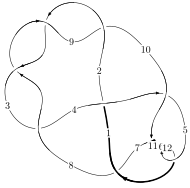
\includegraphics[width=112pt]{../../../GIT/diagram.site/Diagrams/png/1962_12a_1161.png}\\
\ \ \ A knot diagram\footnotemark}&
\allowdisplaybreaks
\textbf{Linearized knot diagam} \\
\cline{2-2}
 &
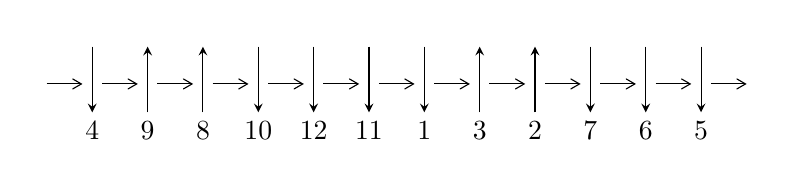
\begin{tikzpicture}[x=20pt, y=17pt]
	% nodes
	\node (C0) at (0, 0) {};
	\node (C1) at (1, 0) {};
	\node (C1U) at (1, +1) {};
	\node (C1D) at (1, -1) {4};

	\node (C2) at (2, 0) {};
	\node (C2U) at (2, +1) {};
	\node (C2D) at (2, -1) {9};

	\node (C3) at (3, 0) {};
	\node (C3U) at (3, +1) {};
	\node (C3D) at (3, -1) {8};

	\node (C4) at (4, 0) {};
	\node (C4U) at (4, +1) {};
	\node (C4D) at (4, -1) {10};

	\node (C5) at (5, 0) {};
	\node (C5U) at (5, +1) {};
	\node (C5D) at (5, -1) {12};

	\node (C6) at (6, 0) {};
	\node (C6U) at (6, +1) {};
	\node (C6D) at (6, -1) {11};

	\node (C7) at (7, 0) {};
	\node (C7U) at (7, +1) {};
	\node (C7D) at (7, -1) {1};

	\node (C8) at (8, 0) {};
	\node (C8U) at (8, +1) {};
	\node (C8D) at (8, -1) {3};

	\node (C9) at (9, 0) {};
	\node (C9U) at (9, +1) {};
	\node (C9D) at (9, -1) {2};

	\node (C10) at (10, 0) {};
	\node (C10U) at (10, +1) {};
	\node (C10D) at (10, -1) {7};

	\node (C11) at (11, 0) {};
	\node (C11U) at (11, +1) {};
	\node (C11D) at (11, -1) {6};

	\node (C12) at (12, 0) {};
	\node (C12U) at (12, +1) {};
	\node (C12D) at (12, -1) {5};
	\node (C13) at (13, 0) {};

	% arrows
	\draw[->,>={angle 60}]
	(C0) edge (C1) (C1) edge (C2) (C2) edge (C3) (C3) edge (C4) (C4) edge (C5) (C5) edge (C6) (C6) edge (C7) (C7) edge (C8) (C8) edge (C9) (C9) edge (C10) (C10) edge (C11) (C11) edge (C12) (C12) edge (C13) ;	\draw[->,>=stealth]
	(C1U) edge (C1D) (C2D) edge (C2U) (C3D) edge (C3U) (C4U) edge (C4D) (C5U) edge (C5D) (C6U) edge (C6D) (C7U) edge (C7D) (C8D) edge (C8U) (C9D) edge (C9U) (C10U) edge (C10D) (C11U) edge (C11D) (C12U) edge (C12D) ;
	\end{tikzpicture} \\
\hhline{~~} \\& 
\textbf{Solving Sequence} \\ \cline{2-2} 
 &
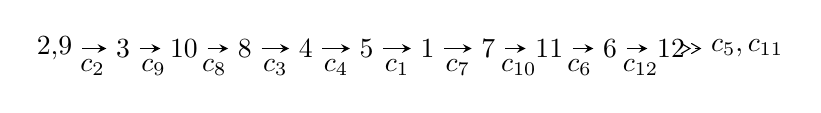
\begin{tikzpicture}[x=22pt, y=7pt]
	% node
	\node (A0) at (-1/8, 0) {2,9};
	\node (A1) at (1, 0) {3};
	\node (A2) at (2, 0) {10};
	\node (A3) at (3, 0) {8};
	\node (A4) at (4, 0) {4};
	\node (A5) at (5, 0) {5};
	\node (A6) at (6, 0) {1};
	\node (A7) at (7, 0) {7};
	\node (A8) at (8, 0) {11};
	\node (A9) at (9, 0) {6};
	\node (A10) at (10, 0) {12};
	\node (C1) at (1/2, -1) {$c_{2}$};
	\node (C2) at (3/2, -1) {$c_{9}$};
	\node (C3) at (5/2, -1) {$c_{8}$};
	\node (C4) at (7/2, -1) {$c_{3}$};
	\node (C5) at (9/2, -1) {$c_{4}$};
	\node (C6) at (11/2, -1) {$c_{1}$};
	\node (C7) at (13/2, -1) {$c_{7}$};
	\node (C8) at (15/2, -1) {$c_{10}$};
	\node (C9) at (17/2, -1) {$c_{6}$};
	\node (C10) at (19/2, -1) {$c_{12}$};
	\node (A11) at (45/4, 0) {$c_{5},c_{11}$};

	% edge
	\draw[->,>=stealth]	
	(A0) edge (A1) (A1) edge (A2) (A2) edge (A3) (A3) edge (A4) (A4) edge (A5) (A5) edge (A6) (A6) edge (A7) (A7) edge (A8) (A8) edge (A9) (A9) edge (A10) ;
	\draw[->>,>={angle 60}]	
	(A10) edge (A11);
\end{tikzpicture} \\ 

\end{tabular} \\

\footnotetext{
The image of knot diagram is generated by the software ``\textbf{Draw programme}" developed by Andrew Bartholomew(\url{http://www.layer8.co.uk/maths/draw/index.htm\#Running-draw}), where we modified some parts for our purpose(\url{https://github.com/CATsTAILs/LinksPainter}).
}\phantom \\ \newline 
\centering \textbf{Ideals for irreducible components\footnotemark of $X_{\text{par}}$} 
 
\begin{align*}
I^u_{1}&=\langle 
u^{32}- u^{31}+\cdots+3 u^2+1\rangle \\
I^u_{2}&=\langle 
u^5+3 u^3+u-1\rangle \\
\\
\end{align*}
\raggedright * 2 irreducible components of $\dim_{\mathbb{C}}=0$, with total 37 representations.\\
\footnotetext{All coefficients of polynomials are rational numbers. But the coefficients are sometimes approximated in decimal forms when there is not enough margin.}
\newpage
\renewcommand{\arraystretch}{1}
\centering \section*{I. $I^u_{1}= \langle u^{32}- u^{31}+\cdots+3 u^2+1 \rangle$}
\flushleft \textbf{(i) Arc colorings}\\
\begin{tabular}{m{7pt} m{180pt} m{7pt} m{180pt} }
\flushright $a_{2}=$&$\begin{pmatrix}1\\0\end{pmatrix}$ \\
\flushright $a_{9}=$&$\begin{pmatrix}0\\u\end{pmatrix}$ \\
\flushright $a_{3}=$&$\begin{pmatrix}1\\- u^2\end{pmatrix}$ \\
\flushright $a_{10}=$&$\begin{pmatrix}u\\u\end{pmatrix}$ \\
\flushright $a_{8}=$&$\begin{pmatrix}- u\\u^3+u\end{pmatrix}$ \\
\flushright $a_{4}=$&$\begin{pmatrix}u^2+1\\- u^4-2 u^2\end{pmatrix}$ \\
\flushright $a_{5}=$&$\begin{pmatrix}u^6+3 u^4+2 u^2+1\\u^6+2 u^4- u^2\end{pmatrix}$ \\
\flushright $a_{1}=$&$\begin{pmatrix}u^6+3 u^4+2 u^2+1\\- u^8-4 u^6-4 u^4\end{pmatrix}$ \\
\flushright $a_{7}=$&$\begin{pmatrix}u^{11}+6 u^9+12 u^7+10 u^5+5 u^3\\- u^{13}-7 u^{11}-17 u^9-16 u^7-4 u^5+u^3+u\end{pmatrix}$ \\
\flushright $a_{11}=$&$\begin{pmatrix}- u^{25}-14 u^{23}+\cdots+5 u^5+u\\u^{27}+15 u^{25}+\cdots+u^3+u\end{pmatrix}$ \\
\flushright $a_{6}=$&$\begin{pmatrix}u^{24}+13 u^{22}+\cdots- u^2- u\\- u^{31}-18 u^{29}+\cdots-2 u^2- u\end{pmatrix}$ \\
\flushright $a_{12}=$&$\begin{pmatrix}- u^{20}-11 u^{18}+\cdots+3 u^2+1\\- u^{20}-10 u^{18}-38 u^{16}-66 u^{14}-47 u^{12}-4 u^{10}+6 u^8+2 u^6-5 u^4\end{pmatrix}$\\&\end{tabular}
\flushleft \textbf{(ii) Obstruction class $= -1$}\\~\\
\flushleft \textbf{(iii) Cusp Shapes $= -4 u^{30}+4 u^{29}-76 u^{28}+68 u^{27}-632 u^{26}+500 u^{25}-3012 u^{24}+2072 u^{23}-9052 u^{22}+5284 u^{21}-17812 u^{20}+8508 u^{19}-23164 u^{18}+8580 u^{17}-19788 u^{16}+5292 u^{15}-10868 u^{14}+1960 u^{13}-3384 u^{12}+344 u^{11}-36 u^{10}-80 u^9+376 u^8-44 u^7+156 u^6-96 u^5+36 u^4-12 u^3-28 u^2+4 u-10$}\\~\\
\newpage\renewcommand{\arraystretch}{1}
\flushleft \textbf{(iv) u-Polynomials at the component}\newline \\
\begin{tabular}{m{50pt}|m{274pt}}
Crossings & \hspace{64pt}u-Polynomials at each crossing \\
\hline $$\begin{aligned}c_{1}\end{aligned}$$&$\begin{aligned}
&u^{32}-9 u^{31}+\cdots-110 u+33
\end{aligned}$\\
\hline $$\begin{aligned}c_{2},c_{3},c_{8}\\c_{9}\end{aligned}$$&$\begin{aligned}
&u^{32}+u^{31}+\cdots+3 u^2+1
\end{aligned}$\\
\hline $$\begin{aligned}c_{4},c_{7}\end{aligned}$$&$\begin{aligned}
&u^{32}-4 u^{31}+\cdots-108 u+36
\end{aligned}$\\
\hline $$\begin{aligned}c_{5},c_{6},c_{10}\\c_{11},c_{12}\end{aligned}$$&$\begin{aligned}
&u^{32}+u^{31}+\cdots+2 u+1
\end{aligned}$\\
\hline
\end{tabular}\\~\\
\newpage\renewcommand{\arraystretch}{1}
\flushleft \textbf{(v) Riley Polynomials at the component}\newline \\
\begin{tabular}{m{50pt}|m{274pt}}
Crossings & \hspace{64pt}Riley Polynomials at each crossing \\
\hline $$\begin{aligned}c_{1}\end{aligned}$$&$\begin{aligned}
&y^{32}-7 y^{31}+\cdots-3982 y+1089
\end{aligned}$\\
\hline $$\begin{aligned}c_{2},c_{3},c_{8}\\c_{9}\end{aligned}$$&$\begin{aligned}
&y^{32}+37 y^{31}+\cdots+6 y+1
\end{aligned}$\\
\hline $$\begin{aligned}c_{4},c_{7}\end{aligned}$$&$\begin{aligned}
&y^{32}-20 y^{31}+\cdots+19080 y+1296
\end{aligned}$\\
\hline $$\begin{aligned}c_{5},c_{6},c_{10}\\c_{11},c_{12}\end{aligned}$$&$\begin{aligned}
&y^{32}+41 y^{31}+\cdots+6 y+1
\end{aligned}$\\
\hline
\end{tabular}\\~\\
\newpage\flushleft \textbf{(vi) Complex Volumes and Cusp Shapes}
$$\begin{array}{c|c|c}  
\text{Solutions to }I^u_{1}& \I (\text{vol} + \sqrt{-1}CS) & \text{Cusp shape}\\
 \hline 
\begin{aligned}
u &= \phantom{-}0.300810 + 0.836112 I\end{aligned}
 & \phantom{-}6.82102 - 1.42764 I & -4.51155 - 0.98064 I \\ \hline\begin{aligned}
u &= \phantom{-}0.300810 - 0.836112 I\end{aligned}
 & \phantom{-}6.82102 + 1.42764 I & -4.51155 + 0.98064 I \\ \hline\begin{aligned}
u &= \phantom{-}0.489031 + 0.734239 I\end{aligned}
 & \phantom{-}8.08609 + 8.05482 I & -2.31310 - 6.73676 I \\ \hline\begin{aligned}
u &= \phantom{-}0.489031 - 0.734239 I\end{aligned}
 & \phantom{-}8.08609 - 8.05482 I & -2.31310 + 6.73676 I \\ \hline\begin{aligned}
u &= -0.454853 + 0.736272 I\end{aligned}
 & -0.91691 - 6.31171 I & -4.12363 + 8.39972 I \\ \hline\begin{aligned}
u &= -0.454853 - 0.736272 I\end{aligned}
 & -0.91691 + 6.31171 I & -4.12363 - 8.39972 I \\ \hline\begin{aligned}
u &= \phantom{-}0.408575 + 0.750241 I\end{aligned}
 & -3.78730 + 3.13913 I & -10.07435 - 5.21729 I \\ \hline\begin{aligned}
u &= \phantom{-}0.408575 - 0.750241 I\end{aligned}
 & -3.78730 - 3.13913 I & -10.07435 + 5.21729 I \\ \hline\begin{aligned}
u &= -0.508887 + 0.453816 I\end{aligned}
 & \phantom{-}12.96460 - 1.76928 I & \phantom{-}2.67390 + 3.90594 I \\ \hline\begin{aligned}
u &= -0.508887 - 0.453816 I\end{aligned}
 & \phantom{-}12.96460 + 1.76928 I & \phantom{-}2.67390 - 3.90594 I \\ \hline\begin{aligned}
u &= \phantom{-}0.431538 + 0.445802 I\end{aligned}
 & \phantom{-}3.53431 + 1.54706 I & \phantom{-}2.87219 - 5.01991 I \\ \hline\begin{aligned}
u &= \phantom{-}0.431538 - 0.445802 I\end{aligned}
 & \phantom{-}3.53431 - 1.54706 I & \phantom{-}2.87219 + 5.01991 I \\ \hline\begin{aligned}
u &= \phantom{-}0.598654 + 0.128367 I\end{aligned}
 & \phantom{-}9.86359 - 4.36101 I & \phantom{-}1.36134 + 2.03096 I \\ \hline\begin{aligned}
u &= \phantom{-}0.598654 - 0.128367 I\end{aligned}
 & \phantom{-}9.86359 + 4.36101 I & \phantom{-}1.36134 - 2.03096 I \\ \hline\begin{aligned}
u &= -0.554088 + 0.092280 I\end{aligned}
 & \phantom{-}0.95148 + 2.86543 I & \phantom{-}0.05561 - 3.87784 I \\ \hline\begin{aligned}
u &= -0.554088 - 0.092280 I\end{aligned}
 & \phantom{-}0.95148 - 2.86543 I & \phantom{-}0.05561 + 3.87784 I \\ \hline\begin{aligned}
u &= -0.09682 + 1.49663 I\end{aligned}
 & \phantom{-}6.60174 - 3.81122 I & \phantom{-0.000000 -}0. + 2.89590 I \\ \hline\begin{aligned}
u &= -0.09682 - 1.49663 I\end{aligned}
 & \phantom{-}6.60174 + 3.81122 I & \phantom{-0.000000 } 0. - 2.89590 I \\ \hline\begin{aligned}
u &= -0.188661 + 0.441864 I\end{aligned}
 & -0.184695 - 0.792115 I & -5.07140 + 8.68136 I \\ \hline\begin{aligned}
u &= -0.188661 - 0.441864 I\end{aligned}
 & -0.184695 + 0.792115 I & -5.07140 - 8.68136 I \\ \hline\begin{aligned}
u &= \phantom{-}0.06894 + 1.52078 I\end{aligned}
 & -2.97865 + 3.12510 I & -4.00000 - 3.93405 I \\ \hline\begin{aligned}
u &= \phantom{-}0.06894 - 1.52078 I\end{aligned}
 & -2.97865 - 3.12510 I & -4.00000 + 3.93405 I \\ \hline\begin{aligned}
u &= -0.02317 + 1.55273 I\end{aligned}
 & -7.06597 - 1.36583 I & \phantom{-0.000000 -}0. + 4.57803 I \\ \hline\begin{aligned}
u &= -0.02317 - 1.55273 I\end{aligned}
 & -7.06597 + 1.36583 I & \phantom{-0.000000 } 0. - 4.57803 I \\ \hline\begin{aligned}
u &= -0.13063 + 1.61792 I\end{aligned}
 & -8.94709 - 8.50994 I & \phantom{-0.000000 } 0 \\ \hline\begin{aligned}
u &= -0.13063 - 1.61792 I\end{aligned}
 & -8.94709 + 8.50994 I & \phantom{-0.000000 } 0 \\ \hline\begin{aligned}
u &= \phantom{-}0.14214 + 1.61709 I\end{aligned}
 & \phantom{-}0.08629 + 10.42610 I & \phantom{-0.000000 } 0 \\ \hline\begin{aligned}
u &= \phantom{-}0.14214 - 1.61709 I\end{aligned}
 & \phantom{-}0.08629 - 10.42610 I & \phantom{-0.000000 } 0 \\ \hline\begin{aligned}
u &= \phantom{-}0.11670 + 1.62115 I\end{aligned}
 & -11.89960 + 5.11913 I & \phantom{-0.000000 } 0 \\ \hline\begin{aligned}
u &= \phantom{-}0.11670 - 1.62115 I\end{aligned}
 & -11.89960 - 5.11913 I & \phantom{-0.000000 } 0\\
 \hline 
 \end{array}$$\newpage$$\begin{array}{c|c|c}  
\text{Solutions to }I^u_{1}& \I (\text{vol} + \sqrt{-1}CS) & \text{Cusp shape}\\
 \hline 
\begin{aligned}
u &= -0.09928 + 1.62252 I\end{aligned}
 & -9.83905 - 1.68285 I & \phantom{-0.000000 } 0 \\ \hline\begin{aligned}
u &= -0.09928 - 1.62252 I\end{aligned}
 & -9.83905 + 1.68285 I & \phantom{-0.000000 } 0\\
 \hline 
 \end{array}$$\newpage\newpage\renewcommand{\arraystretch}{1}
\centering \section*{II. $I^u_{2}= \langle u^5+3 u^3+u-1 \rangle$}
\flushleft \textbf{(i) Arc colorings}\\
\begin{tabular}{m{7pt} m{180pt} m{7pt} m{180pt} }
\flushright $a_{2}=$&$\begin{pmatrix}1\\0\end{pmatrix}$ \\
\flushright $a_{9}=$&$\begin{pmatrix}0\\u\end{pmatrix}$ \\
\flushright $a_{3}=$&$\begin{pmatrix}1\\- u^2\end{pmatrix}$ \\
\flushright $a_{10}=$&$\begin{pmatrix}u\\u\end{pmatrix}$ \\
\flushright $a_{8}=$&$\begin{pmatrix}- u\\u^3+u\end{pmatrix}$ \\
\flushright $a_{4}=$&$\begin{pmatrix}u^2+1\\- u^4-2 u^2\end{pmatrix}$ \\
\flushright $a_{5}=$&$\begin{pmatrix}u^2+u+1\\- u^4-2 u^2+u\end{pmatrix}$ \\
\flushright $a_{1}=$&$\begin{pmatrix}u^2+u+1\\- u^3+u^2- u\end{pmatrix}$ \\
\flushright $a_{7}=$&$\begin{pmatrix}u^2+1\\u^2\end{pmatrix}$ \\
\flushright $a_{11}=$&$\begin{pmatrix}- u^3\\- u^3+u\end{pmatrix}$ \\
\flushright $a_{6}=$&$\begin{pmatrix}u^4+u^2+1\\u^4\end{pmatrix}$ \\
\flushright $a_{12}=$&$\begin{pmatrix}- u^3+1\\-2 u^3-2 u+1\end{pmatrix}$\\&\end{tabular}
\flushleft \textbf{(ii) Obstruction class $= -1$}\\~\\
\flushleft \textbf{(iii) Cusp Shapes $= -6$}\\~\\
\newpage\renewcommand{\arraystretch}{1}
\flushleft \textbf{(iv) u-Polynomials at the component}\newline \\
\begin{tabular}{m{50pt}|m{274pt}}
Crossings & \hspace{64pt}u-Polynomials at each crossing \\
\hline $$\begin{aligned}c_{1}\end{aligned}$$&$\begin{aligned}
&u^5-2 u^4- u^3+4 u^2+3 u-3
\end{aligned}$\\
\hline $$\begin{aligned}c_{2},c_{3},c_{5}\\c_{6},c_{8},c_{9}\\c_{10},c_{11},c_{12}\end{aligned}$$&$\begin{aligned}
&u^5+3 u^3+u+1
\end{aligned}$\\
\hline $$\begin{aligned}c_{4},c_{7}\end{aligned}$$&$\begin{aligned}
&(u+1)^5
\end{aligned}$\\
\hline
\end{tabular}\\~\\
\newpage\renewcommand{\arraystretch}{1}
\flushleft \textbf{(v) Riley Polynomials at the component}\newline \\
\begin{tabular}{m{50pt}|m{274pt}}
Crossings & \hspace{64pt}Riley Polynomials at each crossing \\
\hline $$\begin{aligned}c_{1}\end{aligned}$$&$\begin{aligned}
&y^5-6 y^4+23 y^3-34 y^2+33 y-9
\end{aligned}$\\
\hline $$\begin{aligned}c_{2},c_{3},c_{5}\\c_{6},c_{8},c_{9}\\c_{10},c_{11},c_{12}\end{aligned}$$&$\begin{aligned}
&y^5+6 y^4+11 y^3+6 y^2+y-1
\end{aligned}$\\
\hline $$\begin{aligned}c_{4},c_{7}\end{aligned}$$&$\begin{aligned}
&(y-1)^5
\end{aligned}$\\
\hline
\end{tabular}\\~\\
\newpage\flushleft \textbf{(vi) Complex Volumes and Cusp Shapes}
$$\begin{array}{c|c|c}  
\text{Solutions to }I^u_{2}& \I (\text{vol} + \sqrt{-1}CS) & \text{Cusp shape}\\
 \hline 
\begin{aligned}
u &= -0.343105 + 0.770791 I\end{aligned}
 & -1.64493\phantom{ +0.000000I} & -6.00000\phantom{ +0.000000I} \\ \hline\begin{aligned}
u &= -0.343105 - 0.770791 I\end{aligned}
 & -1.64493\phantom{ +0.000000I} & -6.00000\phantom{ +0.000000I} \\ \hline\begin{aligned}
u &= \phantom{-}0.525261\phantom{ +0.000000I}\end{aligned}
 & -1.64493\phantom{ +0.000000I} & -6.00000\phantom{ +0.000000I} \\ \hline\begin{aligned}
u &= \phantom{-}0.08047 + 1.63341 I\end{aligned}
 & -1.64493\phantom{ +0.000000I} & -6.00000\phantom{ +0.000000I} \\ \hline\begin{aligned}
u &= \phantom{-}0.08047 - 1.63341 I\end{aligned}
 & -1.64493\phantom{ +0.000000I} & -6.00000\phantom{ +0.000000I}\\
 \hline 
 \end{array}$$\newpage
\newpage\renewcommand{\arraystretch}{1}
\centering \section*{ III. u-Polynomials}
\begin{tabular}{m{50pt}|m{274pt}}
Crossings & \hspace{64pt}u-Polynomials at each crossing \\
\hline $$\begin{aligned}c_{1}\end{aligned}$$&$\begin{aligned}
&(u^5-2 u^4- u^3+4 u^2+3 u-3)(u^{32}-9 u^{31}+\cdots-110 u+33)
\end{aligned}$\\
\hline $$\begin{aligned}c_{2},c_{3},c_{8}\\c_{9}\end{aligned}$$&$\begin{aligned}
&(u^5+3 u^3+u+1)(u^{32}+u^{31}+\cdots+3 u^2+1)
\end{aligned}$\\
\hline $$\begin{aligned}c_{4},c_{7}\end{aligned}$$&$\begin{aligned}
&((u+1)^5)(u^{32}-4 u^{31}+\cdots-108 u+36)
\end{aligned}$\\
\hline $$\begin{aligned}c_{5},c_{6},c_{10}\\c_{11},c_{12}\end{aligned}$$&$\begin{aligned}
&(u^5+3 u^3+u+1)(u^{32}+u^{31}+\cdots+2 u+1)
\end{aligned}$\\
\hline
\end{tabular}\newpage\renewcommand{\arraystretch}{1}
\centering \section*{ IV. Riley Polynomials}
\begin{tabular}{m{50pt}|m{274pt}}
Crossings & \hspace{64pt}Riley Polynomials at each crossing \\
\hline $$\begin{aligned}c_{1}\end{aligned}$$&$\begin{aligned}
&(y^5-6 y^4+23 y^3-34 y^2+33 y-9)(y^{32}-7 y^{31}+\cdots-3982 y+1089)
\end{aligned}$\\
\hline $$\begin{aligned}c_{2},c_{3},c_{8}\\c_{9}\end{aligned}$$&$\begin{aligned}
&(y^5+6 y^4+11 y^3+6 y^2+y-1)(y^{32}+37 y^{31}+\cdots+6 y+1)
\end{aligned}$\\
\hline $$\begin{aligned}c_{4},c_{7}\end{aligned}$$&$\begin{aligned}
&((y-1)^5)(y^{32}-20 y^{31}+\cdots+19080 y+1296)
\end{aligned}$\\
\hline $$\begin{aligned}c_{5},c_{6},c_{10}\\c_{11},c_{12}\end{aligned}$$&$\begin{aligned}
&(y^5+6 y^4+11 y^3+6 y^2+y-1)(y^{32}+41 y^{31}+\cdots+6 y+1)
\end{aligned}$\\
\hline
\end{tabular}
\vskip 2pc
\end{document}